\documentclass[border=3pt,tikz]{standalone}
\usepackage{bm,amsmath}
\usetikzlibrary{patterns,decorations.pathmorphing,decorations.text}
\usetikzlibrary{arrows.meta}
\usetikzlibrary{calc}


\begin{document}

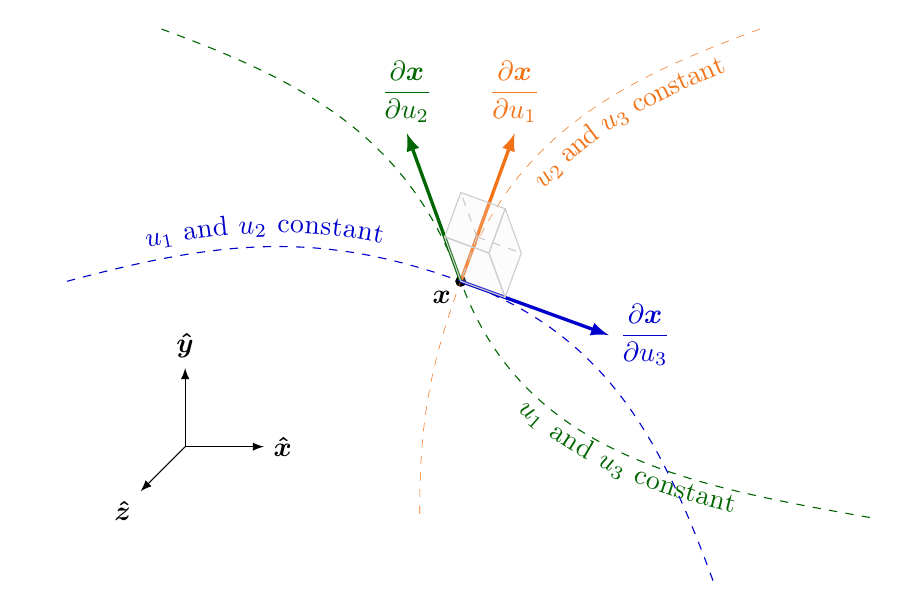
\begin{tikzpicture}[scale=1.0]
    \colorlet{mydarkblue}{blue!80!black}
    \colorlet{myblue}{blue!30}
    \colorlet{mylightblue}{blue!5}
    \colorlet{mydarkred}{red!90!black}
    \colorlet{myred}{red!30}
    \colorlet{mydarkgreen}{green!40!black}
    \colorlet{mygreen}{green!30}
    \colorlet{mydarkorange}{yellow!40!red}
    \colorlet{myorange}{yellow!80!red}
    \colorlet{myyellow}{yellow!80}
    \colorlet{mygrey}{black!25}
    \colorlet{mydarkgrey}{black!70}

    % origin
    \coordinate (O) at (0,0);

    % xyz triplet
    \draw[-latex] (O)--++(0:1) node[right] {$\bm{\hat{x}}$};
    \draw[-latex] (O)--++(90:1) node[above] {$\bm{\hat{y}}$};
    \draw[-latex] (O)--++(225:0.8) node[below left] {$\bm{\hat{z}}$};

    % points for drawing the flow curve
    \coordinate (X_path_start) at ($(O)+(-2,1)$);
    \coordinate (X_path_end) at ($(O)+(9,1)$);

    % define x_t and velocity at x_t
    \path (X_path_start) to[bend left=20] coordinate[pos=0.5] (X_t) (X_path_end);
    \fill (X_t) circle (2pt) node[below left] {$\bm{x}$};
    
    % define u_1-curve and vector
    \draw[-latex,mydarkorange,very thick] (X_t) -- coordinate[pos=0.3] (du_1) ++(70:2) node[above,pos=1] {$\begin{aligned}\frac{\partial\bm{x}}{\partial u_1}\end{aligned}$};
    \draw[dashed,very thin,mydarkorange,,postaction={
    decorate,
    decoration={
        text along path,
        text align=center,
        text={${u_2}$ and ${u_3}$ constant},
        text color=mydarkorange,
        raise=-10pt,
        reverse path=false,
        text align={left indent=1cm},
        }
    },anchor=center] (X_t) to[out=70,in=180+20] ++(40:5);
    \draw[dashed,very thin,mydarkorange] ($(X_t)+(260:3)$) to[out=90,in=180+70] (X_t);

    % define u_2-curve and vector
    \draw[-latex,mydarkgreen,very thick] (X_t) -- coordinate[pos=0.3] (du_2) ++(110:2) node[above,pos=1] {$\begin{aligned}\frac{\partial\bm{x}}{\partial u_2}\end{aligned}$};
    \draw[dashed,mydarkgreen] (X_t) to[out=110,in=180+160] ++(140:5);
    \draw[dashed,mydarkgreen,postaction={
    decorate,
    decoration={
        text along path,
        text align=center,
        text={${u_1}$ and ${u_3}$ constant},
        text color=mydarkgreen,
        raise=-8pt,
        reverse path=true,
        }
    },anchor=center] ($(X_t)+(330:6)$) to[out=170,in=180+110] (X_t);

    
    % define u_3-curve and vector
    \draw[-latex,mydarkblue,very thick] (X_t) -- coordinate[pos=0.3] (du_3) ++(-20:2) node[right,pos=1] {$\begin{aligned}\frac{\partial\bm{x}}{\partial u_3}\end{aligned}$};
    \draw[dashed,mydarkblue] (X_t) to[out=-20,in=180-70] ++(-50:5);
    \draw[dashed,mydarkblue,,postaction={
    decorate,
    decoration={
        text along path,
        text align=center,
        text={${u_1}$ and ${u_2}$ constant},
        text color=mydarkblue,
        raise=5pt,
        reverse path=false,
        }
    },anchor=center] ($(X_t)+(180:5)$) to[out=15,in=180-20] (X_t);

    % draw box faces
    \draw[dashed,mygrey] (du_1)--($(du_1)+(du_2)-(X_t)$);
    \draw[dashed,mygrey] (du_1)--(X_t);
    \draw[dashed,mygrey] (du_1)--($(du_3)+(du_1)-(X_t)$);
    
    \draw[gray!40,fill=gray!10,fill opacity=0.2,line join=bevel] (du_2)--($(du_2)+(du_1)-(X_t)$)--($(du_3)+(du_2)-(X_t)+(du_1)-(X_t)$)--($(du_3)+(du_2)-(X_t)$)--cycle;
    
    \draw[gray!40,fill=gray!10,fill opacity=0.2,line join=bevel] (X_t)--(du_2)--($(du_2)+(du_3)-(X_t)$)--(du_3)--cycle;

    \draw[gray!40,fill=gray!10,fill opacity=0.2,line join=bevel] (du_3)--($(du_3)+(du_1)-(X_t)$)--($(du_3)+(du_1)-(X_t)+(du_2)-(X_t)$)--($(du_3)+(du_2)-(X_t)$)--cycle;
    
\end{tikzpicture}

\end{document}
